% Section 2 - Core library
% Alessandro Tenaglia <alessandro.tenaglia@uniroma2.it>
% May 6, 2022

% ### Core library ###
\section{Core library}
\graphicspath{{figs/section2/}}

% --- Code organisation ---
\begin{frame}{Code organisation}
	One of the main features of the MARTe2 architecture is the bold separation between:
	\begin{itemize}
		\item<1-> the platform \textbg{architecture}, i.e. x86, armv8;
		\item<2-> the \textbg{environment} details, i.e. Linux, FreeRTOS, Windows;
		\item<3-> the \textbg{real-time algorithms}, i.e. the user code;
	\end{itemize}
\end{frame}

% --- Code organisation ---
\begin{frame}{Code organisation}
	\begin{figure}
		\centering
		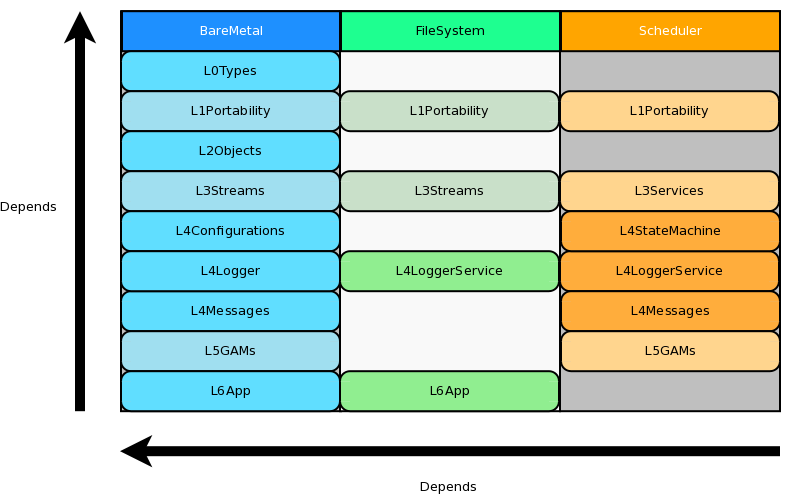
\includegraphics[scale=.35]{Tiers.png}
		\label{fig:tiers}
		\caption{Code library}
	\end{figure}
\end{frame}

% --- Makefile ---
\begin{frame}{Makefile}
	\begin{columns}
		\column{.5\textwidth}
		The build of the core library (and all MARTe2 base projects) follows this structure:
		\begin{itemize}
			\item<1-> The \textbg{Makefile.os-arch} defines the \textbg{TARGET} operating system and architecture;
			\item<2-> The \textbg{Makefile.inc} defines all the common rules;
			\item<3-> The \textbg{MakeDefaults} defines the specific rules for the \textbg{TARGET};
		\end{itemize}
		\column{.5\textwidth}
		\begin{figure}
			\centering
			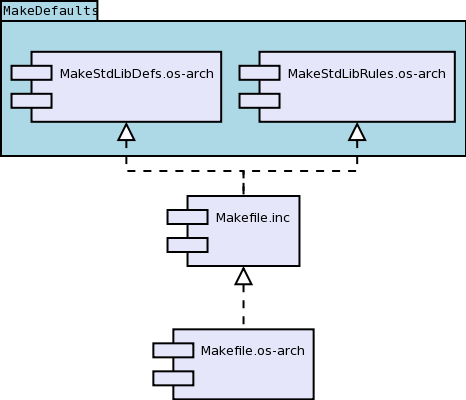
\includegraphics[scale=.3]{Makefiles.png}
			\label{fig:makefiles}
			\caption{Makefile structure, \\ from bottom to top}
		\end{figure}
	\end{columns}
\end{frame}
